\chapter{Handling Millions of Atomic Structures} \label{chap:mpdd}

\acknowledge{
This chapter adapts parts of a manuscript draft planned for publication before dissertation submission, co-authored with Ricardo Amaral, Jonathan W. Siegel, and Zi-Kui Liu. All of included text was written by Adam M. Krajewski. Described software has been developed by Adam M. Krajewski since 2020 with assistance from Jonathan W. Siegel and Ricardo Amaral. Zi-Kui Liu provided edits and guidance. It also adapts excerpt written by Adam M. Krajewski for \citet{Evans2024DevelopmentsExchange} reproduced from Digital Discovery journal under CC BY 3.0 license. 
}


\section{Introduction} \label{mpdd:sec:background}

A



\section{The Material-Property-Descriptor Database} \label{mpdd:sec:mpdd}

\subsection{Motivation} \label{mpdd:ssec:motivation}

The Material-Property-Descriptor Database (MPDD) is an extensive (4.5M+) database of \emph{ab initio} relaxations of 3D crystal structures,  combined with an infrastructure of tools allowing efficient descriptor calculation (featurization), as well as the deployment of ML models like \texttt{SIPFENN} \cite{Krajewski2024EfficientStructures} described in Chapter \ref{chap:sipfenn}, and other developed by the community.

The most critical motivation behind MPDD is the retention of intermediate modeling data (atomistic features features), including structure-informed descriptors described in Chapter \ref{chap:pysipfenn}, which typically cost orders of magnitude more computational time than any of the other steps performed during ML model deployment~\cite{Krajewski2022ExtensibleNetworks}. Thus, many ML models can be run at a small fraction of the original cost if the same descriptor (or, more commonly, a subset chosen through feature selection) is used. This benefit applies regardless of whether a model is just another iteration, e.g., fine-tuned to a specific class of materials like perovskites, or an entirely new model for a different property.

Thus, machine learning researchers can effortlessly take advantage of MPDD to deploy numerous ML models directly to the community without needing to construct individual deployment targets, which are typically both much smaller and redundant relative to existing datasets.

Furthermore, MPDD's access to stored atomic structures and associated metadata has been shown to be useful, for instance, in the fully data-driven prediction of atomic structures (validated with DFT and experiments). It, for instance allowed quick identification of unknown structures in Nd-Bi~\cite{Im2022ThermodynamicModeling} and Al-Fe~\cite{Shang2021FormingJoints} systems, what is discussed in more detail in Chapter \ref{chap:crystall}.

\subsection{Design Philosophy} \label{mpdd:ssec:designphilosophy}

\begin{figure}[H]
    \centering
    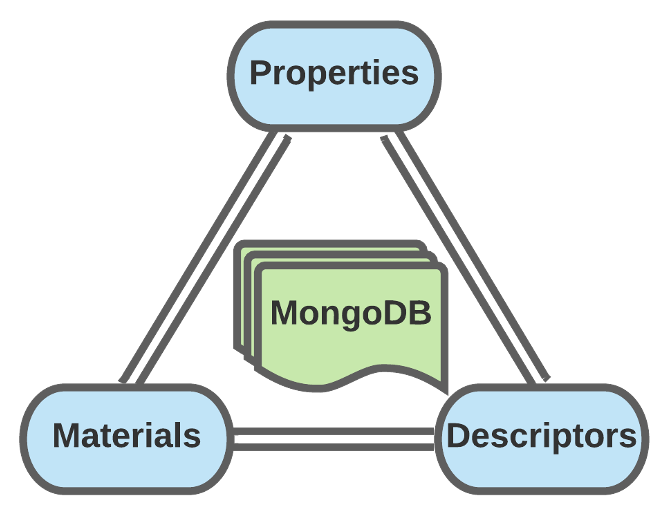
\includegraphics[width=0.4\textwidth]{mpdd/MPDD_CoreTriplet.png}
    \caption{Three entities at the core of MPDD treated as "first class citizens" interacting with each other. Going counter-clockwise \emph{Materials} cover our past sampling of the problem domain, \emph{Descriptors} cover our understanding of it, and \emph{Properties} determine utility. Going clockwise desired \emph{Properties} guide analysis leading to understanding encoded in \emph{Descriptors}, which inform us of unexplored regions of problem domain in their individual contexts.}
    \label{mpdd:fig:core}
\end{figure}



\subsection{Dataset} \label{mpdd:ssec:dataset}

DFT-based databases including OQMD \cite{Saal2013MaterialsOQMD, Kirklin2015TheEnergies, Shen2022ReflectionsOQMD}, AFLOW \cite{Curtarolo2013AFLOW:Discovery, Toher2018TheDiscovery}, Materials Project \cite{Jain2013Commentary:Innovation}, NIST-JARVIS \cite{Choudhary2020TheDesign}, Alexandria \cite{Schmidt2022AFunctionals}, CAMD \cite{Ye2022NovelAgents}, GNoME \cite{Merchant2023ScalingDiscovery}, and in-house datasets including phonon calculations created with DFTTK \cite{Wang2021DFTTK:Calculations}. Hundreds of thousands of experimentally observed entries from Crystallography Open Database (COD) \cite{Grazulis2009CrystallographyStructures, Grazulis2012CrystallographyCollaboration, Grazulis2019CrystallographyPerspectives}.


\begin{figure}[H]
    \centering
    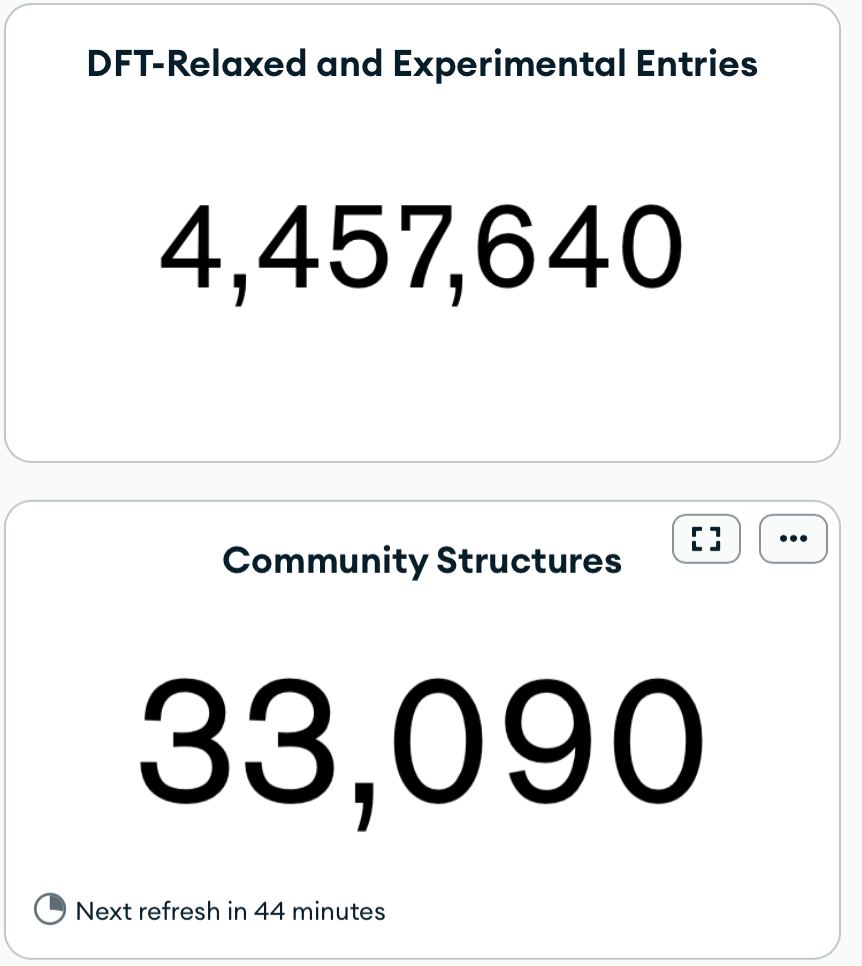
\includegraphics[width=0.4\textwidth]{mpdd/Screenshot 2024-05-05 at 11.54.32.png}
    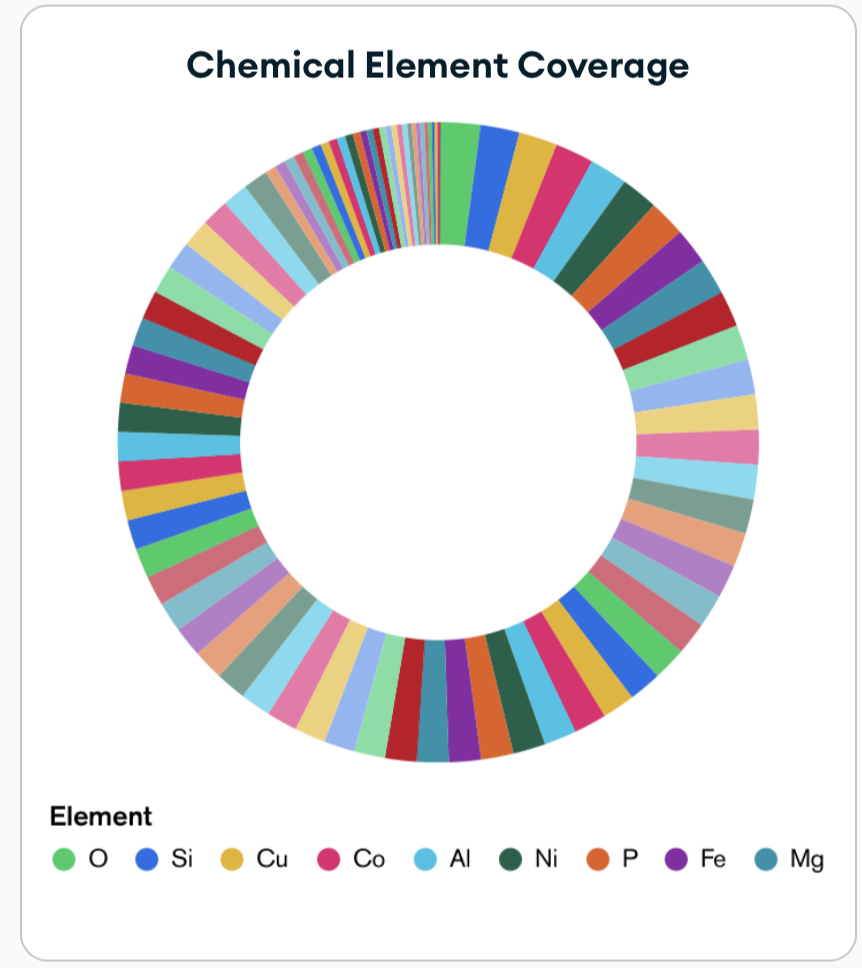
\includegraphics[width=0.4\textwidth]{mpdd/Screenshot 2024-05-05 at 11.54.47.png}
    \caption{Key statistics over MPDD dataset as of April 2024 demonstrating (1) extent of the dataset and (2) high diversity of chemical space coverage over all elements.}
    \label{mpdd:fig:dataset}
\end{figure}

\subsection{Infrastructure} \label{mpdd:ssec:infrastructure}

\todo

\begin{figure}[H]
    \centering
    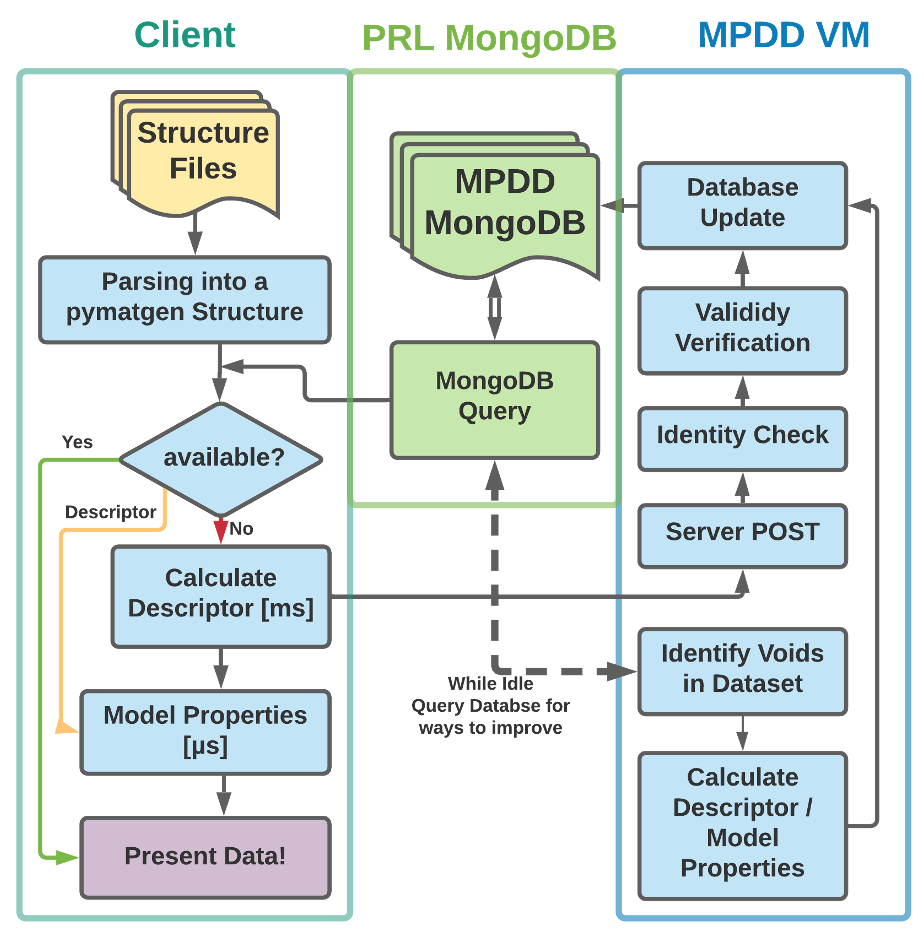
\includegraphics[width=0.4\textwidth]{mpdd/mpdd_core.png}
    \caption{Main schematic of the MPDD Database }
    \label{mpdd:fig:schematic}
\end{figure}


\section{MPDD-eXchange} \label{mpdd:sec:mpddx}

\todo

\begin{figure}[H]
    \centering
    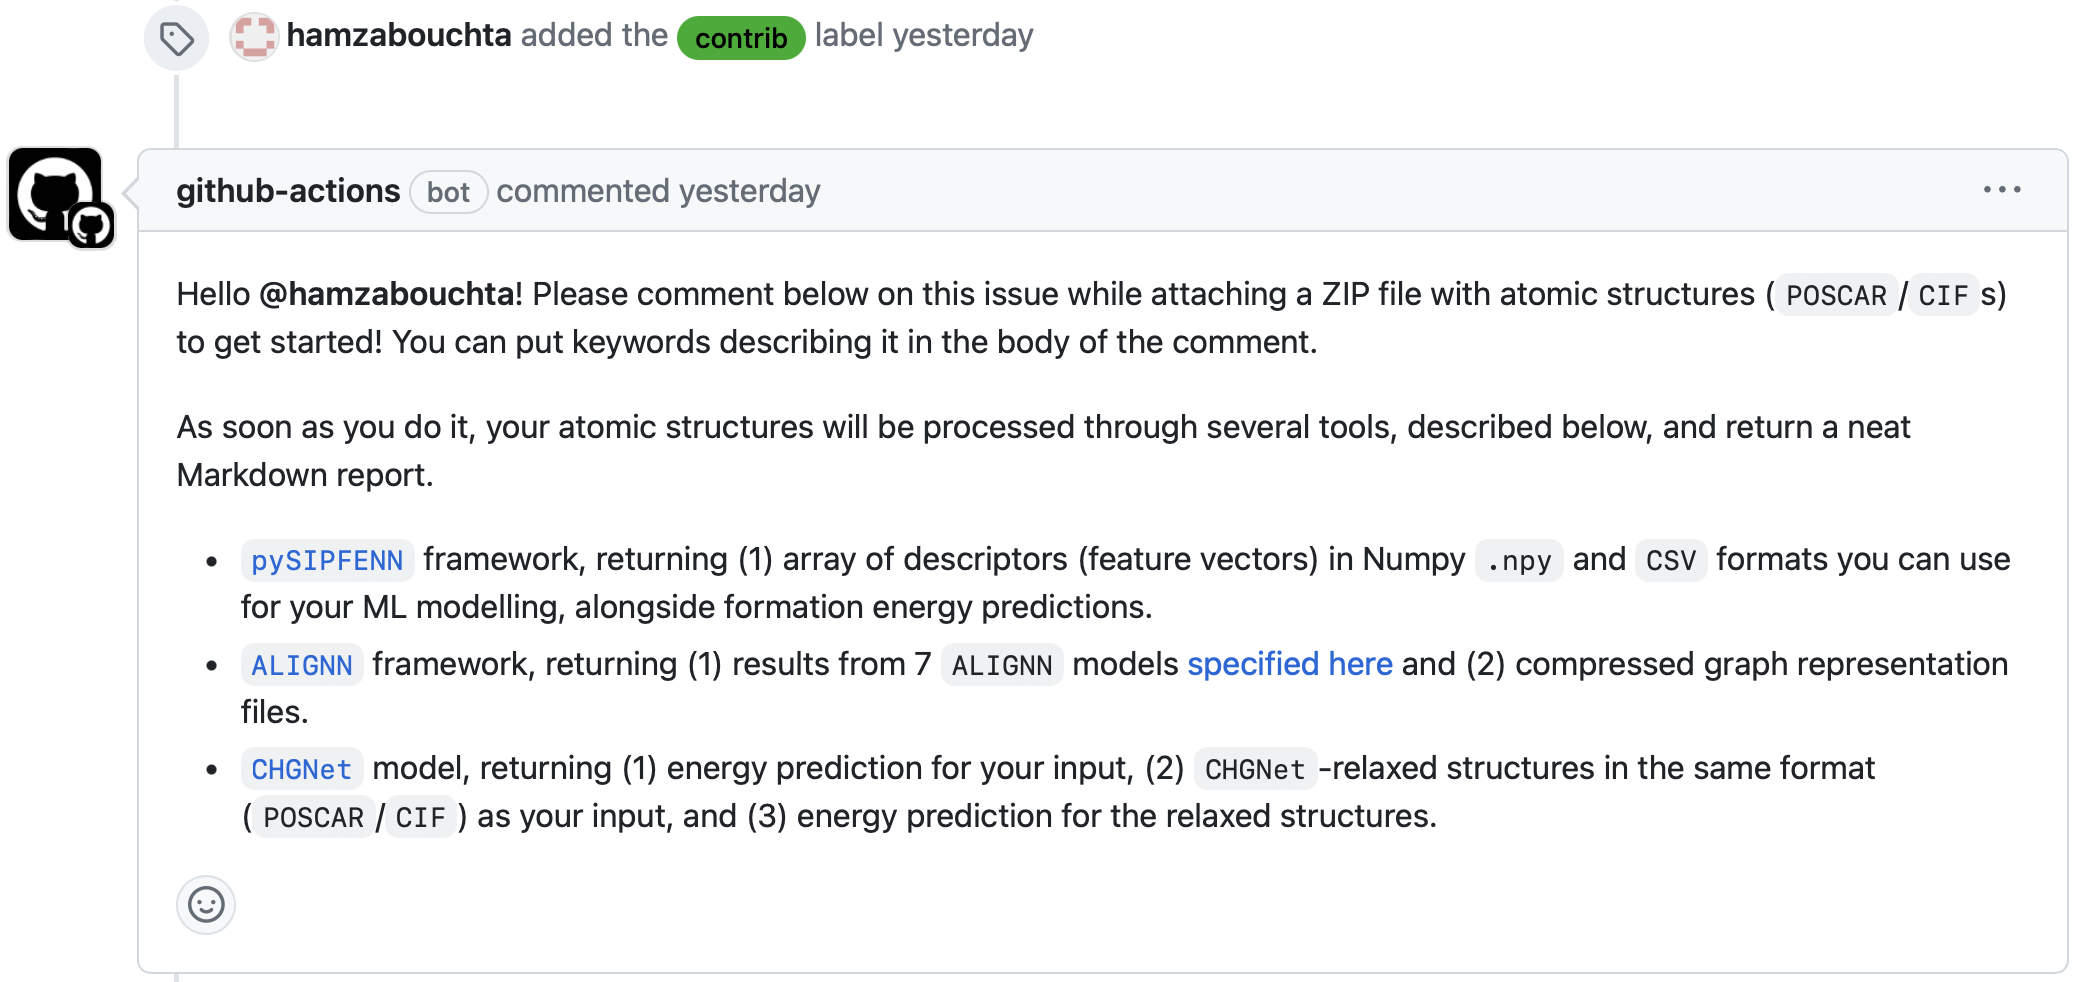
\includegraphics[width=0.7\textwidth]{mpdd/mpddx1.png}
    \caption{Printout of the greeting message on issues opened with auto-assigned \texttt{contrib} label instructing user how to send a contribution and what models will be run.}
    \label{mpdd:fig:mpddx1}
\end{figure}

\todo

\begin{figure}[H]
    \centering
    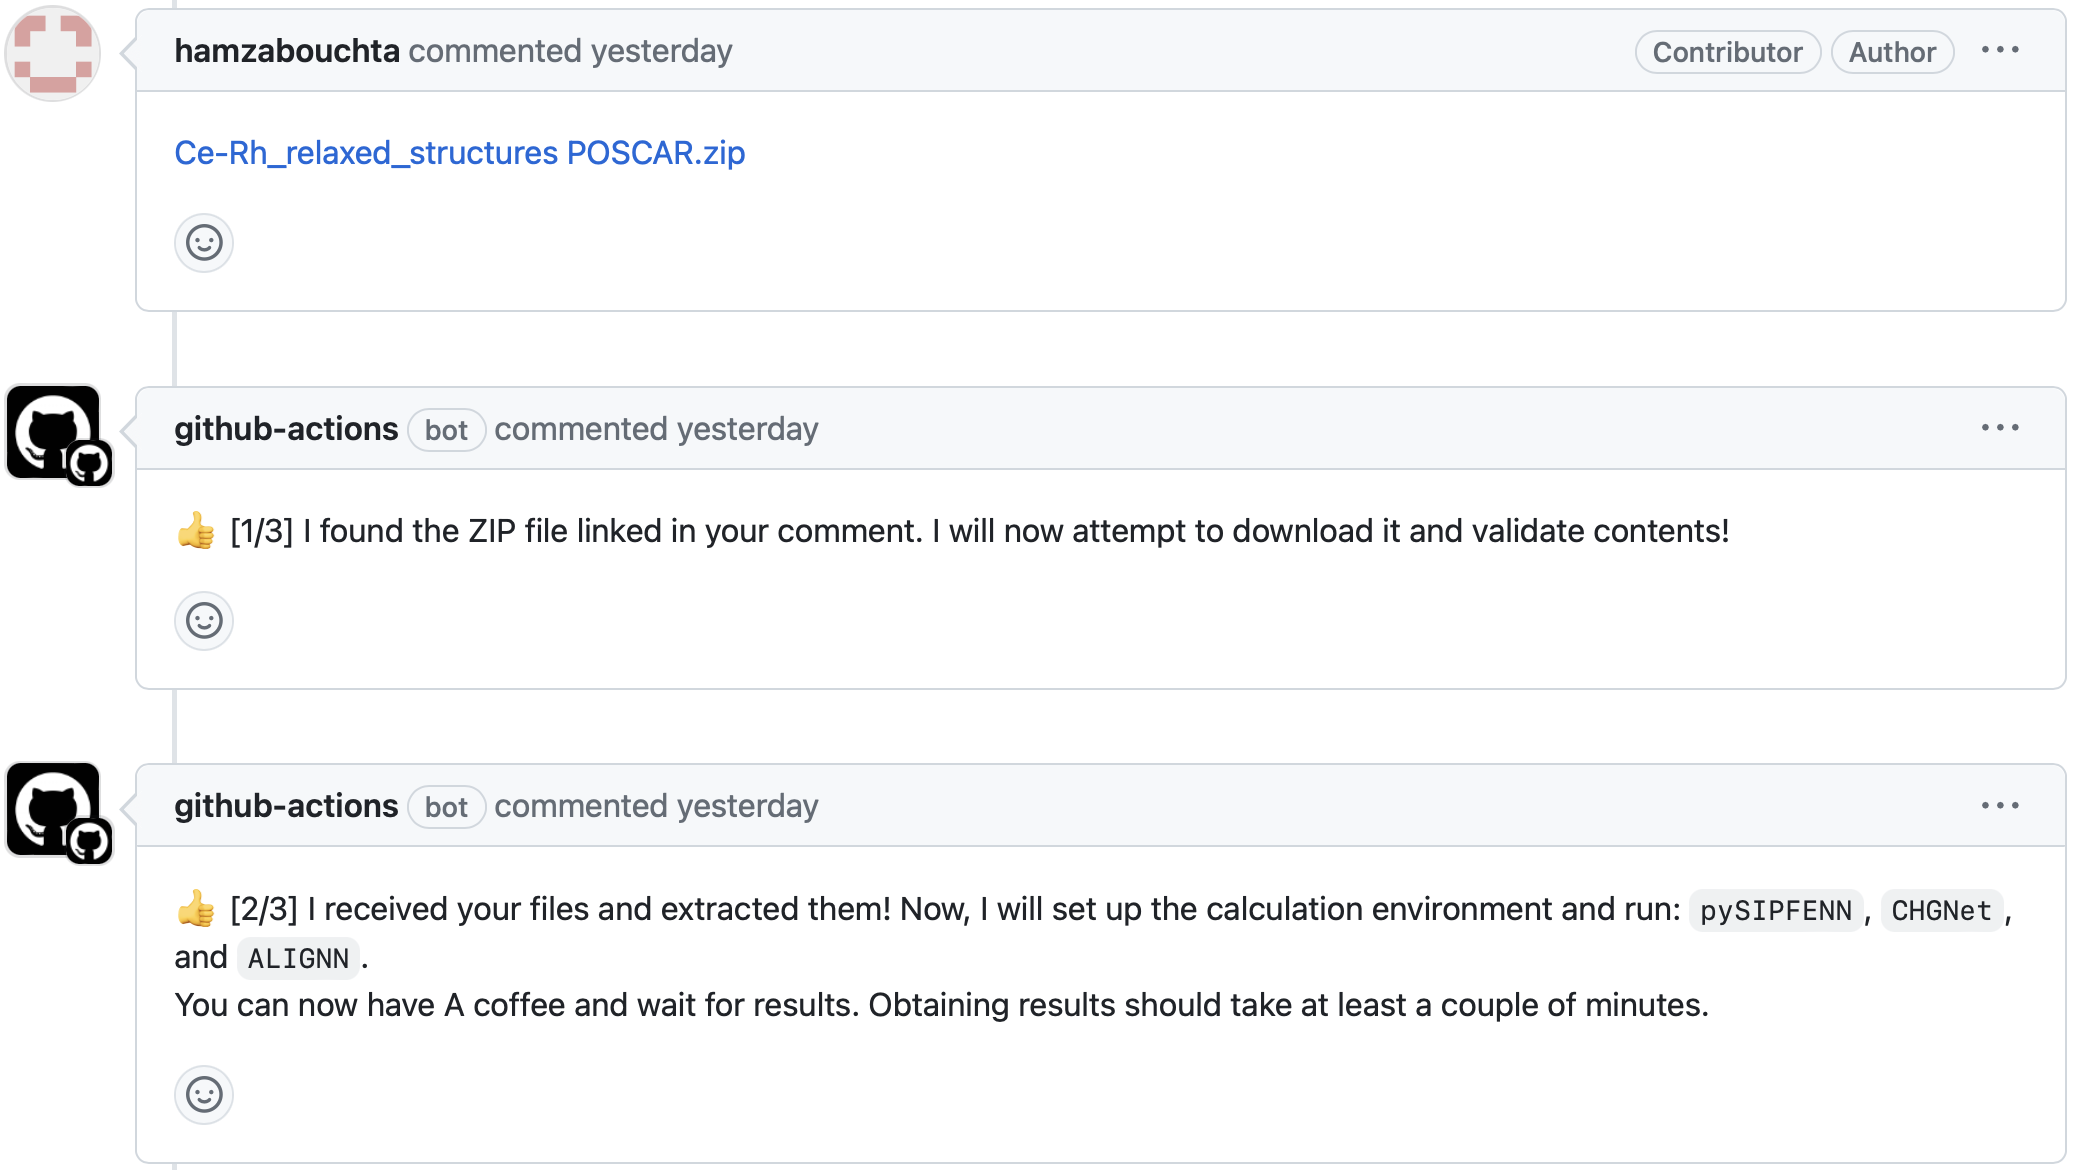
\includegraphics[width=0.7\textwidth]{mpdd/mpddx2.png}
    \caption{Printout of the intermediate messages informing that validation checks are passing, if the user sent a properly formatted CIF or POSCAR files in a ZIP file. Otherwise (not depicted) messages would provide feedback on errors.}
    \label{mpdd:fig:mpddx2}
\end{figure}

\todo

\begin{figure}[H]
    \centering
    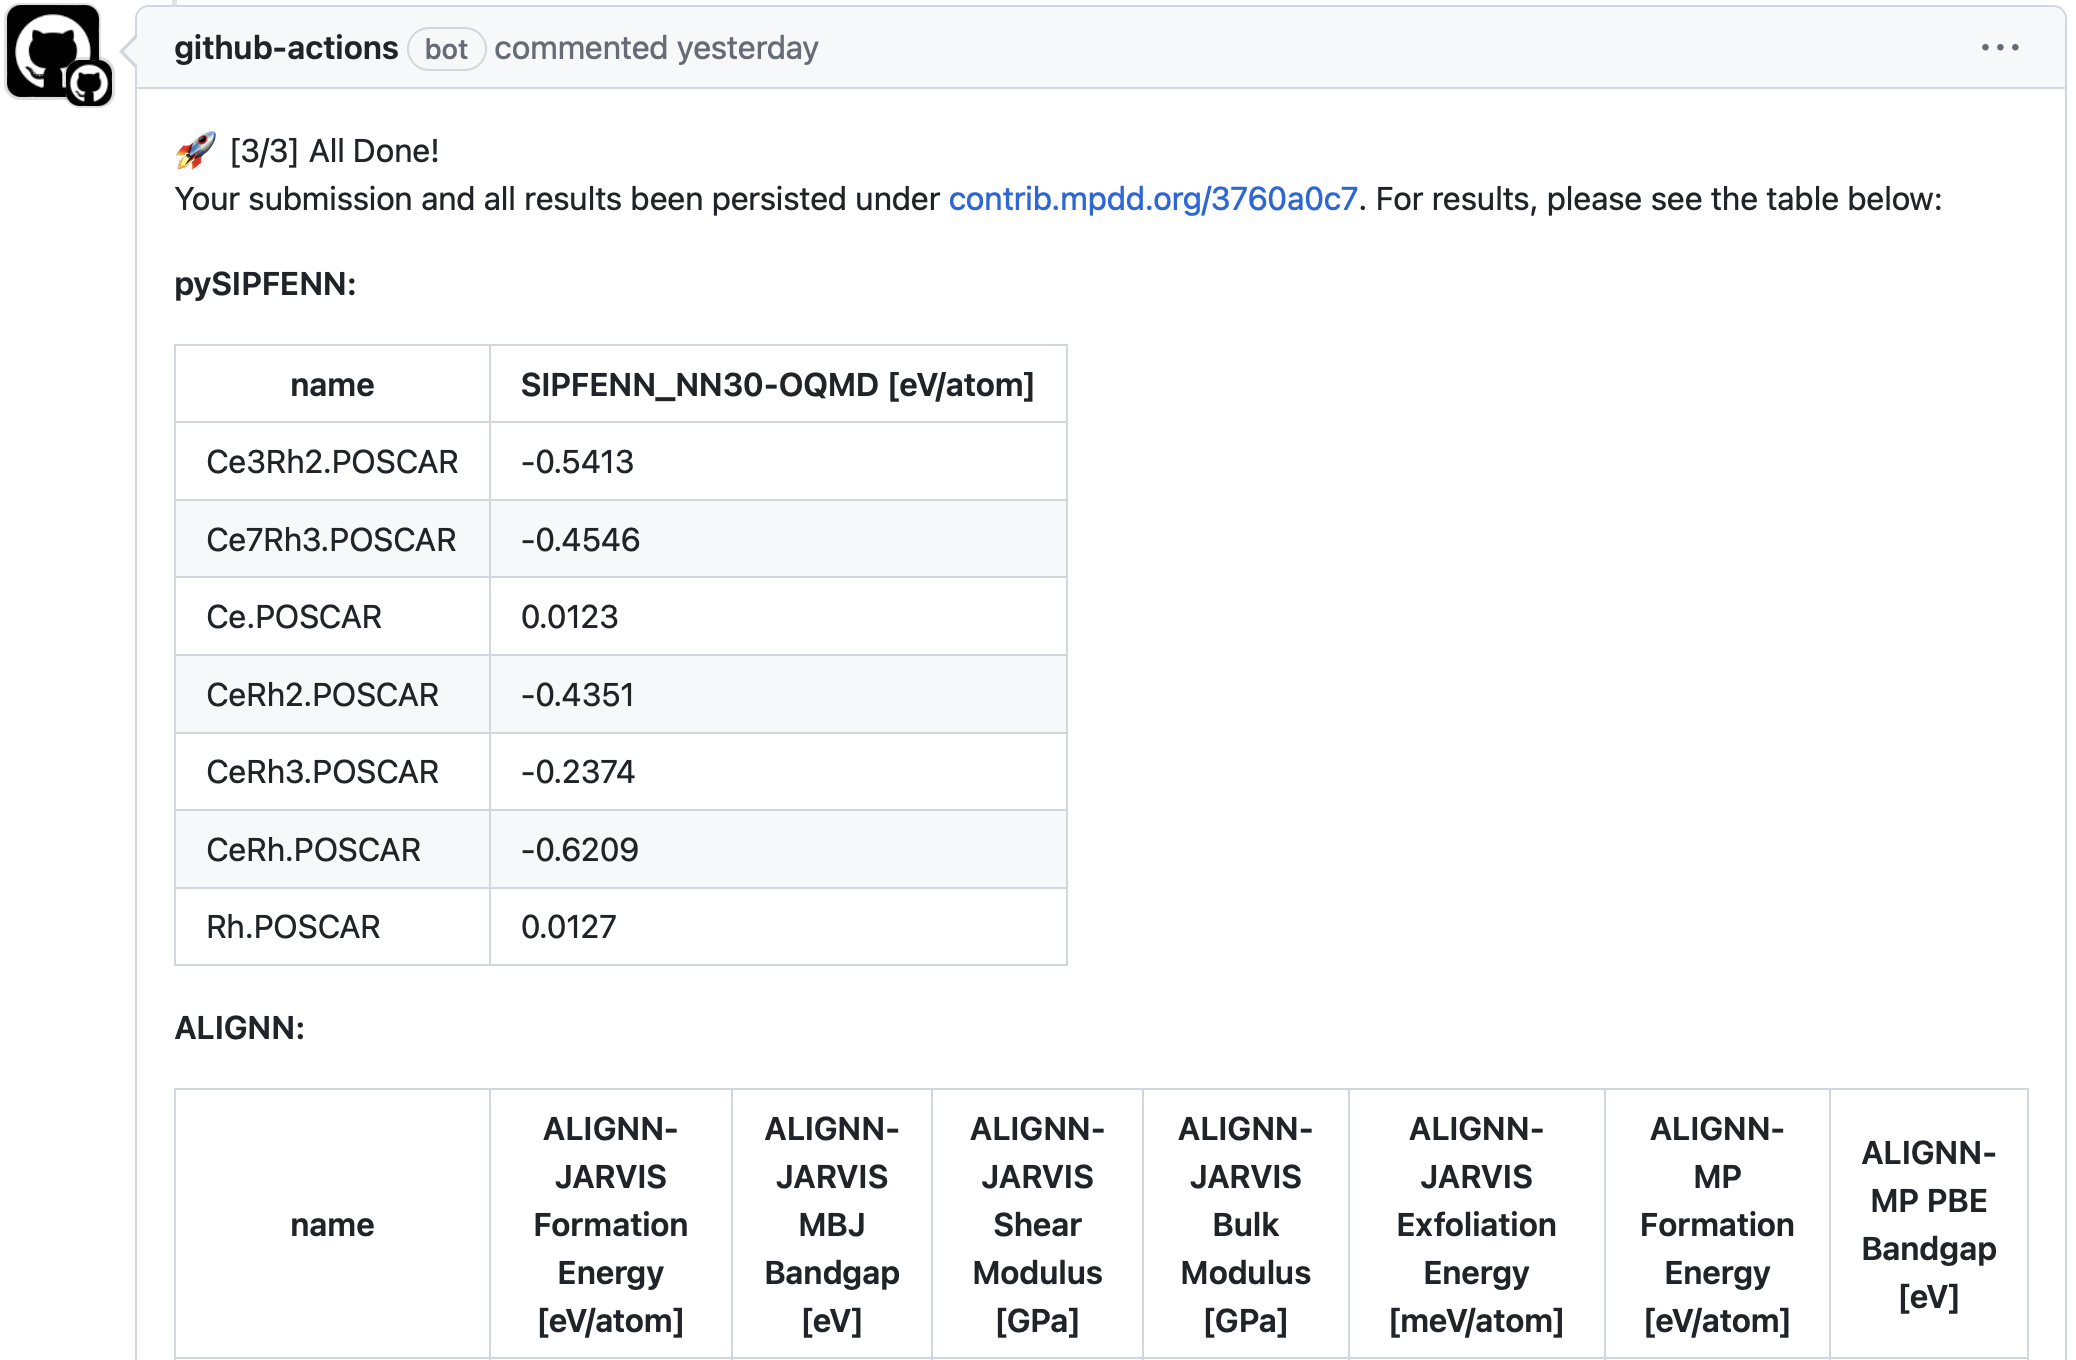
\includegraphics[width=0.7\textwidth]{mpdd/mpddx3.png}
    \caption{Printout of final message after all computation is successfully completed. User is presented with (1) outputs of the ML models deployed on the data and (2) a unique contribution ID based on the commit hash, which can be cited as \texttt{contrib.mpdd.org/3760a0c7} or \texttt{mat-x.org/mpdd-3760a0c7} and points to persisted data record appended with ML results and calculation metadata.}
    \label{mpdd:fig:mpddx3}
\end{figure}


\todo

\begin{figure}[H]
    \centering
    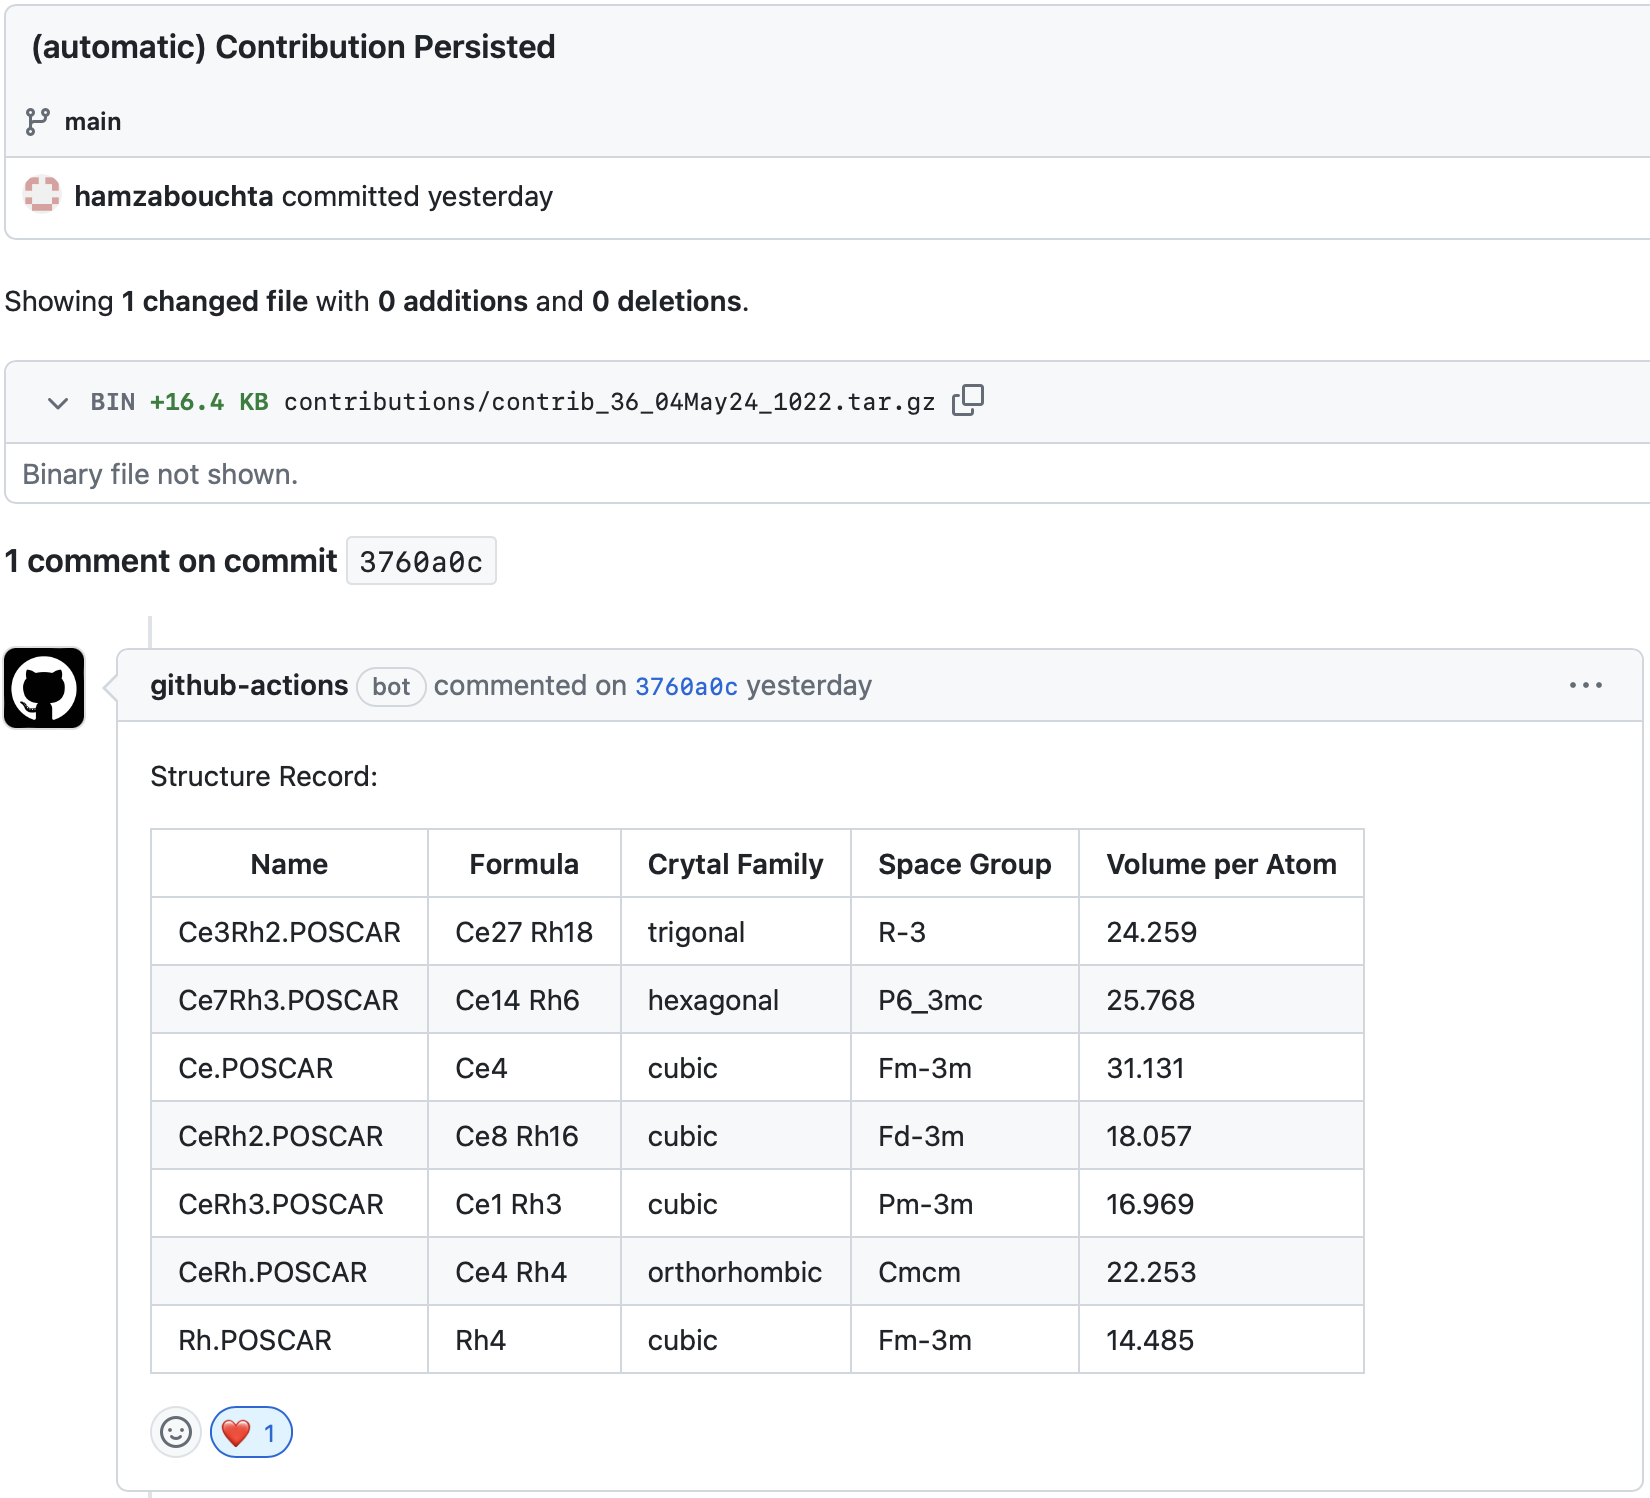
\includegraphics[width=0.75\textwidth]{mpdd/mpddx4.png}
    \caption{Printout of contribution record stored within git repository as auto-generated commit. Right after a successful commit, the system automatically generates a comment on it describing the structures included.}
    \label{mpdd:fig:mpddx4}
\end{figure}




\section{Open Databases Integration for Materials Design (OPTIMADE) API} \label{mpdd:sec:optimade}

\texttt{OPTIMADE} or the Open Databases Integration for Materials Design consortium has been established to make materials databases interoperable by developing a specification for a common REST API \cite{Evans2024DevelopmentsExchange}. That way, databases can remain independently maintained and tuned to specific needs, like ab initio data or ML data, while at the same time reporting on the contained knowledge so that redundant calculations are not performed and the efficiency of the materials informatics community at large is dramatically improved.

MPDD has a stable OPTIMADE API that serves the entire core MPDD dataset, fully implementing \texttt{v1.1.0} of the OPTIMADE standard, as of April 2024, through a cloud server based on \texttt{optimade-python-tools} \cite{Evans2021}.
Making the MPDD available via OPTIMADE was initially challenging, as MPDD stores and exchanges data in a way that prioritises high throughput and low storage requirements, including binary data, making it difficult or slow to make MPDD queryable as an OPTIMADE API on-the-fly.
However, issues have been resolved by establishing a self-updating mirror of the dataset where structures are made OPTIMADE-compliant during transfer, which can occur within the same virtual machine or other integrated computing environment. Most of the MPDD-specific data is available under the \texttt{mpdd} namespace of \texttt{OPTIMADE}, including dictionaries of metadata (e.g., \texttt{\_mpdd\_atomicvolume}), properties (e.g., \texttt{\_mpdd\_formationenergy\_sipfenn\_krajewski2020\_lightmodel}), and descriptors (e.g., \texttt{\_mpdd\_descriptors.KS2022}), described earlier in this chapter.

The base URL is available at:

\hspace{24pt} \href{https://optimade.mpdd.org}{https://optimade.mpdd.org}

and one can see a sample dataset response by following the \texttt{structures} endpoint at:

\hspace{24pt} \href{https://optimade.mpdd.org/v1/structures}{https://optimade.mpdd.org/v1/structures}



\printbibliography[heading=subbibintoc]